\documentclass[12pt]{article}
\usepackage{graphicx}
\usepackage{float}
\usepackage{amsmath}
\title{Experiment 7: Sequence Generator}
\author{Annirudh K P\\%
210070009}
\date{October 3, 2022}
\begin{document}

\maketitle

\section{Overview of the experiment}
\paragraph{}
In this experiment, we started working on sequential circuit designs using structural modelling on VHDL. The problem statement of this experiment is to design a Sequence Generator. The objective of this experiment was to understand the Quartus Design Flow, work with the Xen10 Board, use ScanChain for testbenching, and give us hands on experience over different technical glitches/problems we may face in this piece of software which has been made unwantedly hard.

\section{Experimental Set-up}

\subsection{Design Schematics}
The following design schematics are shown for the Sequence Generator 

\begin{figure}[H]
\centering
  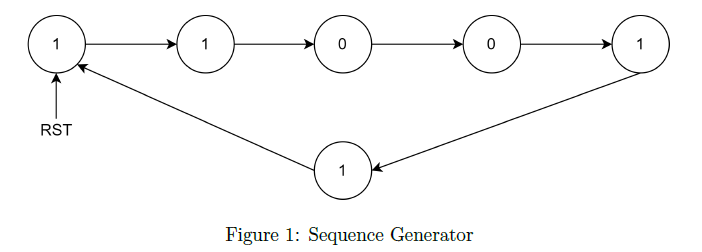
\includegraphics[scale=0.3]{Images/SeqGen_ProbStat.png}
  \caption{}
\end{figure}

\begin{figure}[H]
\centering
  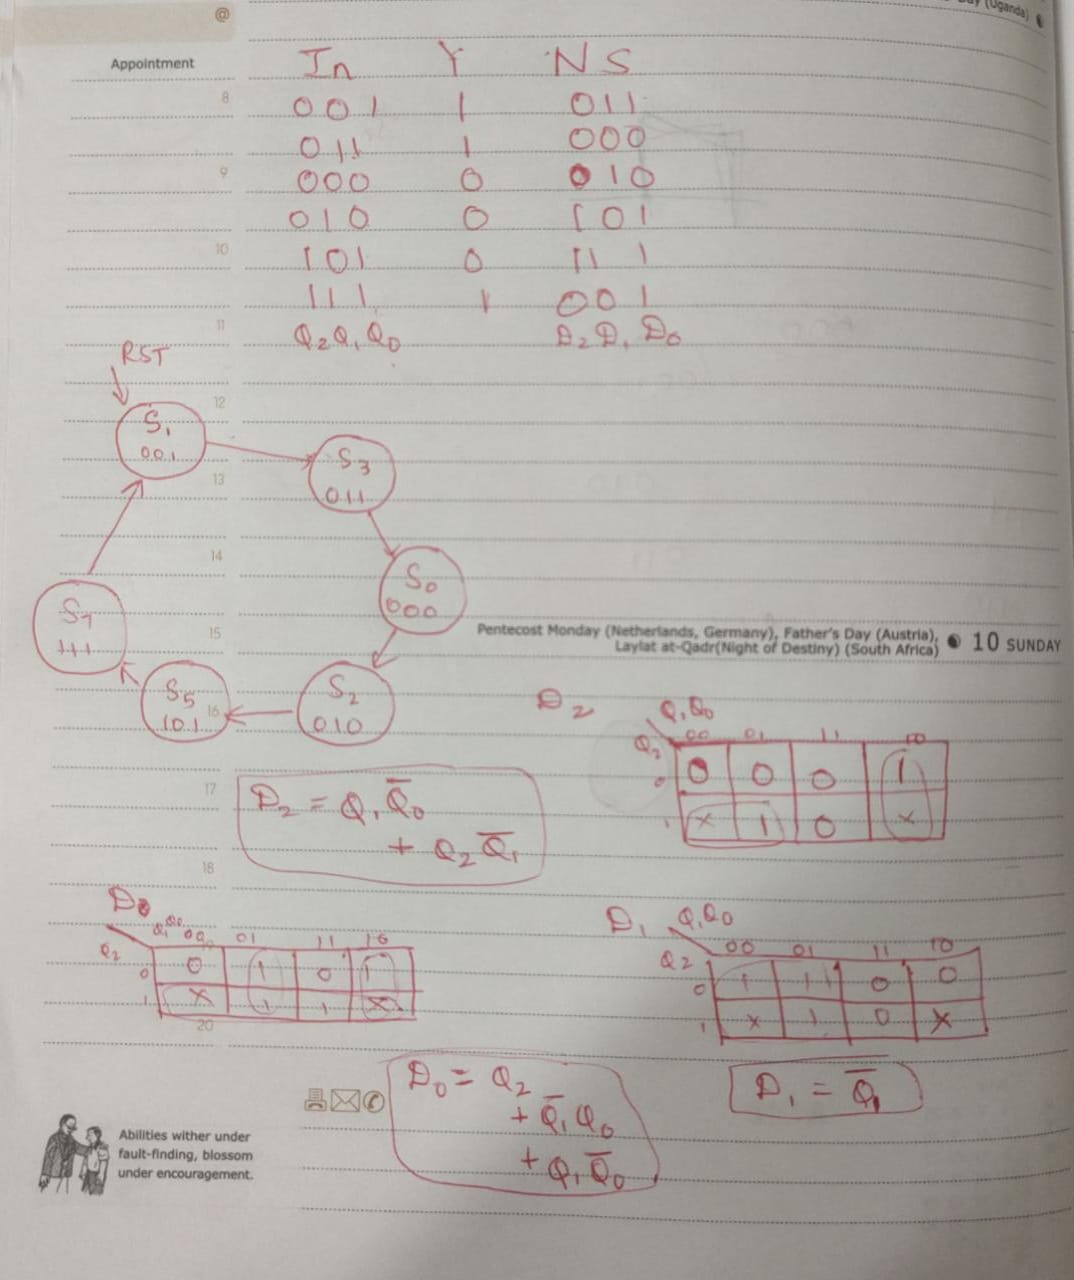
\includegraphics[scale=0.3]{Images/SeqGen_Design.jpeg}
  \caption{}
\end{figure}

\subsection{Description of Components}
\subsubsection{Sequence Generator}
\begin{verbatim}
library ieee;
use ieee.std_logic_1164.all;
package Flipflops is
component dff_set is port(D,clock,set:in std_logic;Q:out std_logic);
end component dff_set;
component dff_reset is port(D,clock,reset:in std_logic;Q:out std_logic);
end component dff_reset;
end package Flipflops;

--D flip flop with set
library ieee;
use ieee.std_logic_1164.all;
entity dff_set is port(D,clock,set:in std_logic;Q:out std_logic);
end entity dff_set;

architecture behav of dff_set is
begin
dff_set_proc: process (clock,set)
begin
if(set='1')then -- set implies flip flip output logic high
Q <= '0'; -- write the flip flop output when set
elsif (clock'event and (clock='1')) then
Q <= D; -- write flip flop output when not set
end if ;
end process dff_set_proc;
end behav;


--D flip flop with reset
library ieee;
use ieee.std_logic_1164.all;
entity dff_reset is port(D,clock,reset:in std_logic;Q:out std_logic);
end entity dff_reset;


architecture behav of dff_reset is
begin
dff_reset_proc: process (clock,reset)
begin
if(reset='1')then -- reset implies flip flip output logic low
Q <= '1'; -- write the flip flop output when reset
elsif (clock'event and (clock='1')) then
Q <= D; -- write flip flop output when not reset
end if ;
end process dff_reset_proc;
end behav;


library ieee;
use ieee.std_logic_1164.all;
-- write the Flipflops packege declaration
entity Sequence_generator_stru_dataflow is
port (reset,clock: in std_logic;
y:out std_logic);
end entity Sequence_generator_stru_dataflow;

architecture struct of Sequence_generator_stru_dataflow is
signal D :std_logic_vector(2 downto 0);
signal Q:std_logic_vector(2 downto 0);
component dff_set is port(D,clock,set:in std_logic;Q:out std_logic);
end component dff_set;
component dff_reset is port(D,clock,reset:in std_logic;Q:out std_logic);
end component dff_reset;
begin
-- write the equations in dataflow e.g z=a+bc written as z <= a or (b and c)
-- for DFF inputs which was derived and also for y.
-- Instantiate components dff_reset
-- and dff_set appropriately using port map statements.
	D(2) <= ((Q(1) and (not Q(0))) or (Q(2) and (not Q(1))));
	D(1) <= (not Q(1));
	D(0) <= (Q(2) or (Q(1) xor Q(0)));
	
	ff1: dff_set port map (D => D(2), clock => clock, set => reset, Q => Q(2));
	ff2: dff_set port map (D => D(1), clock => clock, set => reset, Q => Q(1));
	ff3: dff_reset port map (D => D(0), clock => clock, reset => reset, Q => Q(0));
	y <= Q(0);
end struct;
\end{verbatim}

\section{Observations}
 
We get RTL simulation waveforms for corresponding to input and output which is given below and it shows required results.

\begin{figure}[H]
\centering
  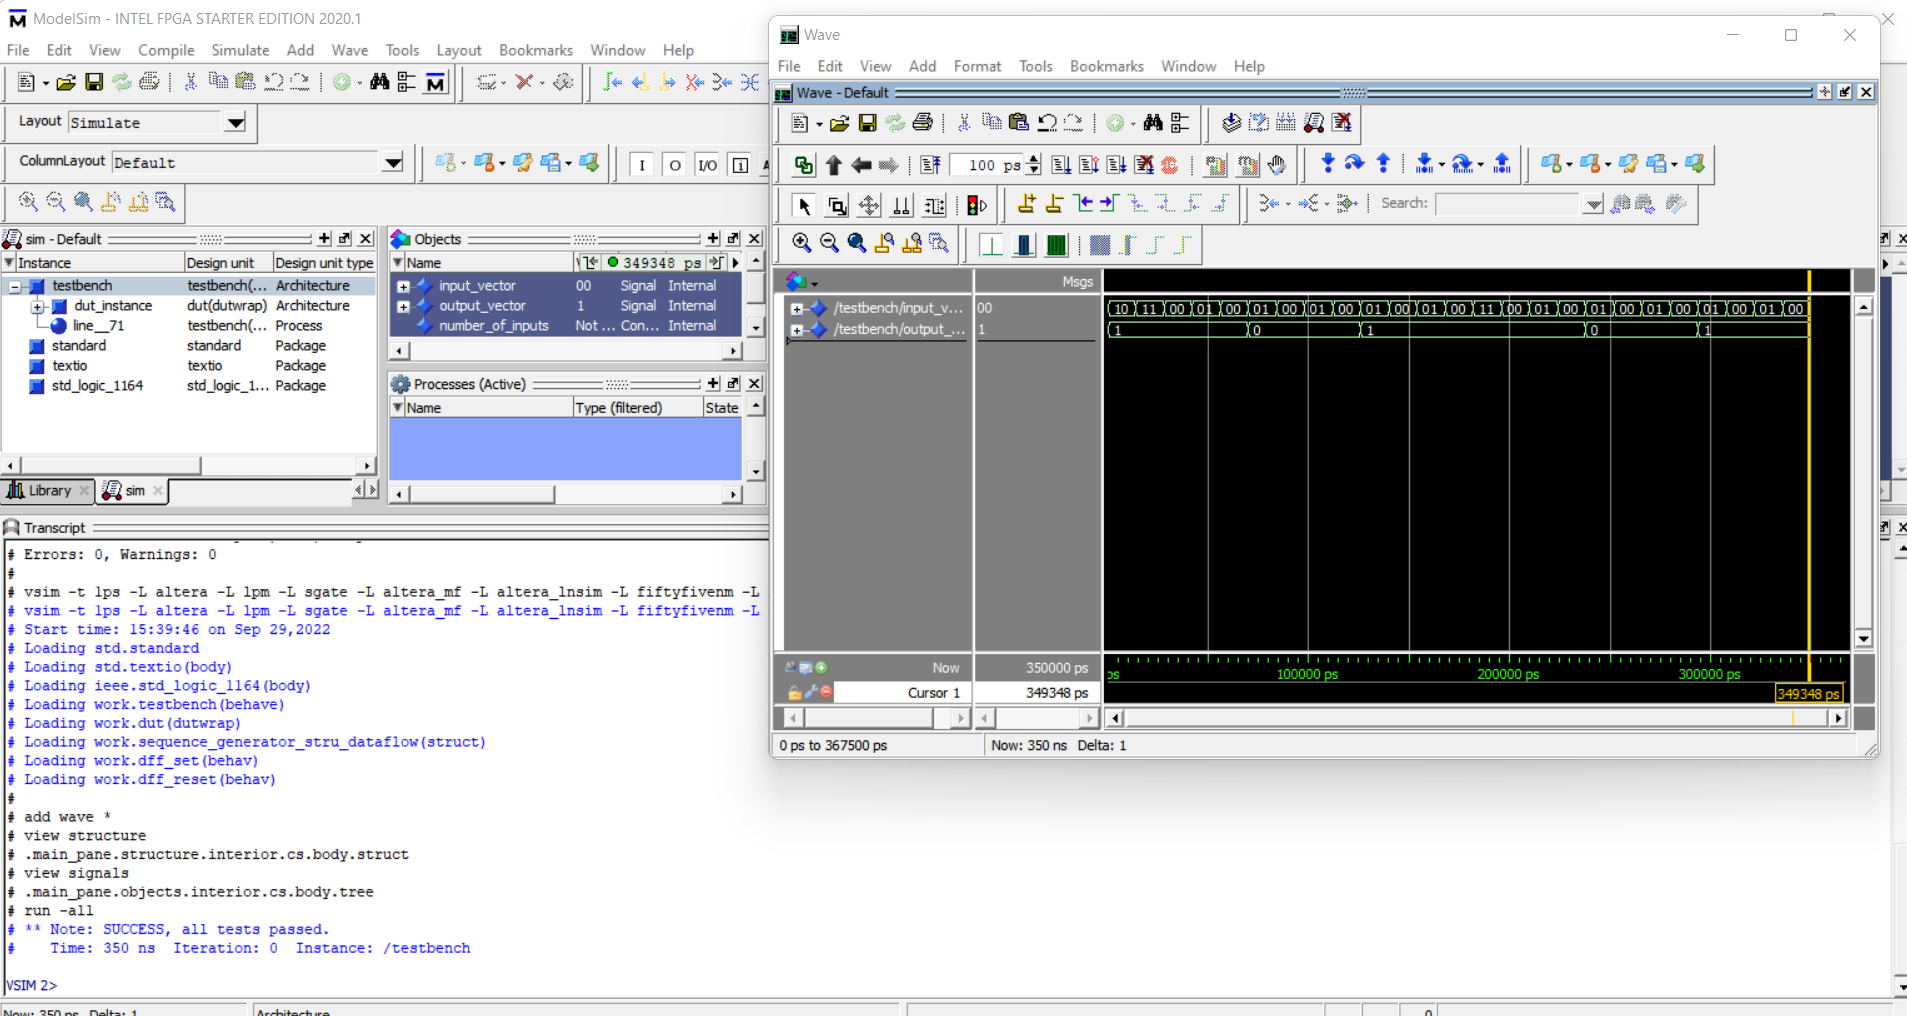
\includegraphics[scale=0.35]{Images/SeqGen_RTLSimulation.png}
  \caption{Sequence Generator RTL Simulation Waveform}
\end{figure}

Further the code (in form of .svf file) was flashed onto the Xen10 board. Then scanchain was run to generate outputs using tracefile and then compared to the golden outputs to check if the outputs were indeed correct. The output was verified, which also verified the working of the logic for the Sequence Generator. The output file's content is shown below.

\begin{verbatim}
10 1 Success
11 1 Success
00 1 Success
01 1 Success
00 1 Success
01 0 Success
00 0 Success
01 0 Success
00 0 Success
01 1 Success
00 1 Success
01 1 Success
00 1 Success
11 1 Success
00 1 Success
01 1 Success
00 1 Success
01 0 Success
00 0 Success
01 0 Success
00 0 Success
01 1 Success
00 1 Success
01 1 Success
00 1 Success
\end{verbatim}

\end{document}